\documentclass[11pt]{article}
\usepackage[margin=0.95in]{geometry}
\usepackage{graphicx}
\usepackage{booktabs}
\usepackage{amsmath,amssymb}
\usepackage[hidelinks]{hyperref}
\usepackage{microtype}
\usepackage{caption}

\title{\textbf{New Directions in Cytochrome P450 Inhibition Modeling:\\
Foundation Language Models, 3D Conformer Geometry,\\
Continuous Potency Supervision, and All-Atom Co-Folding}}
\author{Daniel E. Siegle\\
\footnotesize Standalone Technical Guide \& Frontier Investigation (PubChem AID1851 Benchmark)}
\date{November 2026}

\begin{document}
\maketitle

\begin{abstract}
Whereas the companion ten-year retrospective established what modern tabular, fingerprint, and multi-task neural architectures achieve on PubChem Bioassay AID1851 (reaching 0.8792 mean held-out Test ROC-AUC across CYP 1A2, 2C9, 2C19, 2D6, and 3A4), this standalone study explores \textbf{three frontier directions} from 2025--2026 computational pharmacology: (1)~billion-molecule chemical language modeling (\texttt{MoLFormer-XL}) paired with deterministic 3D conformer geometry (RDKit ETKDGv3), (2)~10-head joint binary + continuous \texttt{ActivityScore} multi-task supervision (\texttt{MT\_Joint3D}), and (3)~targeted all-atom \texttt{Boltz-2} \texttt{[CYP + Heme + Ligand]} 3D co-folding. Written as a didactic first-principles guide, this paper explains \emph{why} each tool was selected (and why generative protein binder-design models do not apply), \emph{how} each method works mathematically, what engineering realities arose, and what the zero-leakage data show.

Fusing 151 3D conformer descriptors, 768-d \texttt{MoLFormer-XL} embeddings, and continuous potency supervision lifts mean held-out Test ROC-AUC to a new benchmark of \textbf{0.8810} (\textbf{80.98\%} mean Accuracy, \textbf{0.1376} Brier; DeLong $p < 0.05$ over Tier 4 on 4/5 isozymes, positive on 5/5), while a \textbf{100\% open-source stack} (zero MOE descriptors) reaches \textbf{0.8799} AUC ($p \in [0.058, 0.547]$ vs.\ All-Modal). On the 100 hardest, highest-uncertainty CYP 1A2 test compounds (50\% on unseen Bemis--Murcko scaffolds), zero-fit rank fusion with all-atom \texttt{Boltz-2} \texttt{[CYP 1A2 + HEM + Ligand]} co-folding jumps ROC-AUC from \textbf{0.6464 to 0.7120 (+0.0656)} overall and from \textbf{0.6144 to 0.7104 (+0.0960)} on novel scaffolds---demonstrating a practical two-tier screening architecture combining fast open-source ML with targeted 3D structural triage.
\end{abstract}

\section{Purpose and Tool Triage: What Transfers to Small-Molecule CYP Modeling?}
A common pitfall in contemporary AI-for-science is assuming that any breakthrough biomolecular model transfers directly to any pharmacology problem. Before launching GPU experiments, we objectively audited the open-source toolset from recent autonomous protein-binder design campaigns (\texttt{RFdiffusion3}, \texttt{FreeBindCraft}, \texttt{BoltzGen}, \texttt{SolubleMPNN}, \texttt{ESMFold2}, \texttt{ESMC}, \texttt{Protenix v2}, \texttt{Chai-1}, \texttt{Boltz-2}):
\begin{itemize}
  \item \textbf{Generative backbone/sequence design} (\texttt{RFdiffusion/3}, \texttt{FreeBindCraft}, \texttt{SolubleMPNN}) solves the \emph{inverse} problem---inventing new proteins. Here, the five human CYP enzymes are fixed and the variable is a small-molecule ligand (SMILES).
  \item \textbf{Protein-only predictors \& PLMs} (\texttt{ESMFold2}, \texttt{ESMC}) cannot encode small molecules or the catalytic Heme-b cofactor.
  \item \textbf{All-atom co-folding (\texttt{Boltz-2})} \emph{does} transfer because it jointly folds \texttt{[CYP sequence + Heme-b (HEM) + ligand SMILES]} with induced-fit active-site remodeling. However, at $\sim$3--4\,min/complex on a Tesla T4 GPU, co-folding all 52,000 AID1851 pairs is compute-prohibitive ($\sim$200+ GPU-hours), pointing to a principled two-tier strategy: fast 3D ligand + chemical-LM upgrades across all 16,725 molecules first, followed by surgical \texttt{Boltz-2} co-folding on the hardest, novel-scaffold test slice.
\end{itemize}

\section{Direction 1: Billion-Molecule \texttt{MoLFormer-XL} \& 3D Conformer Geometry}
\subsection{How \texttt{MoLFormer-XL} Works}
Chemical language models treat SMILES strings as sentences and pretrain via masked-token prediction over massive unlabeled chemical libraries, implicitly learning valence, aromaticity, ring closures, and functional-group context. Upgrading from Tier 3B's compact 3-layer \texttt{ChemBERTa-77M-MTR} (3.4M parameters, 77M molecules) to IBM's 12-layer \texttt{ibm/MoLFormer-XL-both-10pct} (47M parameters, 768-d embeddings, \textbf{1.1 billion} ZINC + PubChem molecules) introduces Rotary Position Embeddings (RoPE) and linear-complexity attention. Crucially, because linear attention's exponential feature map overflows \texttt{float16} (producing \texttt{NaN}s), running in pure \texttt{float32} ($\text{lr}=5\times 10^{-5}$) was essential. On raw SMILES alone (zero descriptors, zero fingerprints), end-to-end 10-head fine-tuning of \texttt{MT\_MoLFormer\_XL} achieved \textbf{0.8694 mean Test AUC} (\textbf{79.65\% Acc}), beating \texttt{ChemBERTa} (+0.0035 AUC) and the entire 186-MOE Tier 1 ensemble (+0.0082 AUC).

\subsection{How RDKit ETKDGv3 3D Conformer Descriptors Work}
2D fingerprints capture bonding topology but cannot directly see 3D molecular shape---such as whether a molecule is flat enough to fit CYP 1A2's narrow planar active-site slot. Using RDKit's deterministic \texttt{ETKDGv3} distance-geometry generator (\texttt{randomSeed=0}), we embedded 3D conformers for \textbf{16,585 / 16,725 (99.16\%)} unique PubChem SIDs and extracted \textbf{151 3D descriptors}: 11 global shape/planarity metrics (including Plane of Best Fit \texttt{PBF}, \texttt{NPR1/2}, \texttt{PMI1--3}, \texttt{Asphericity}, \texttt{RadiusOfGyration}), 60 \texttt{USRCAT} 3D pharmacophore shape moments (all-atom, hydrophobic, aromatic, H-bond donor/acceptor), and 80 \texttt{AUTOCORR3D} spatial autocorrelations.

\section{Direction 2: Joint Binary + Continuous \texttt{ActivityScore} Multi-Tasking}
Standard binary QSAR binarizes $\text{ActivityScore} \ge 40$, discarding the difference between an inert molecule (score 0) and a borderline weak binder (score 38), or between a marginal inhibitor (score 41) and a potent nanomolar inhibitor (score 98). To recover this supervision under our exact double-firewall zero-leakage protocol (purging all \texttt{test\{iso\}} and fold-$k$ \texttt{val\{iso\}} SIDs across all five CYP heads), \texttt{MT\_Joint3D} trains a 10-head Residual MLP ($\text{in\_dim} \to 640 \to 2\times\text{ResBlock}(640) \to 256 \to 10$) over 2D FPs + 151 3D conformers + frozen 768-d \texttt{MoLFormer-XL} embeddings using a masked joint objective ($s_{it} = \text{ActivityScore}_{it}/100$, $w_{t^*}=2.0$, $w_t=1.0$):
\begin{equation}
  \mathcal{L}_{\text{Joint}} = \frac{\sum_{i \in \mathcal{B}} \sum_{t=1}^{5} m_{it}\, w_t \Big[\ell_{\text{BCE}}(\hat{z}_{it}, y_{it}) + 0.6\,\ell_{\text{SmoothL1}}(\hat{s}_{it}, s_{it})\Big]}{\sum_{i \in \mathcal{B}} \sum_{t=1}^{5} m_{it}\, w_t}.
\end{equation}
As a single 100\% open-source model (0 MOE descriptors), \texttt{MT\_Joint3D\_OpenSource} reached \textbf{0.8755 mean Test AUC} (\textbf{80.39\% Acc}). Folding \texttt{MT\_Joint3D} into the nested meta-stack lifted the Tier 5 All-Modal stack and blend to \textbf{0.8810 mean Test AUC} and \textbf{80.98\% mean Acc} (Table~\ref{tab:t5}, Figure~\ref{fig:t5}A), significantly outperforming Tier 4 on 4/5 isozymes (DeLong $p \in [0.0059, 0.044]$; positive on 5/5). Meanwhile, \texttt{Tier5\_OpenSource\_Stack} (0 MOE) hit \textbf{0.8799 AUC}, surpassing Tier 4 All-Modal with proprietary MOE's residual lift remaining non-significant on all five isozymes ($p \in [0.058, 0.547]$).

\begin{table}[htbp]
\centering
\scriptsize
\setlength{\tabcolsep}{4pt}
\caption{Tier 5 held-out test Accuracy / ROC-AUC across all five CYP isozymes (100\% test coverage).}
\label{tab:t5}
\resizebox{\textwidth}{!}{%
\begin{tabular}{lccccccc}
\toprule
Model & 1A2 & 2C9 & 2C19 & 2D6 & 3A4 & Mean Acc & Mean AUC \\
\midrule
\emph{Ref: 2015 \texttt{SVM\_baseline} (MOE)} & 0.806 / 0.886 & 0.745 / 0.816 & 0.774 / 0.845 & 0.749 / 0.830 & 0.746 / 0.831 & 0.7640 & 0.8416 \\
\emph{Ref: Tier 4 \texttt{Grand\_AllModal\_Stack}} & 0.837 / 0.913 & 0.782 / 0.856 & 0.806 / 0.878 & 0.801 / 0.863 & 0.803 / 0.886 & 0.8056 & 0.8792 \\
\midrule
Dir.\ 1: \texttt{MT\_MoLFormer\_XL} (SMILES) & 0.827 / 0.904 & 0.784 / 0.847 & 0.805 / 0.875 & 0.776 / 0.850 & 0.791 / 0.871 & 0.7965 & 0.8694 \\
Dir.\ 2: \texttt{MT\_Joint3D\_OpenSource} (0 MOE) & 0.830 / 0.910 & 0.784 / 0.853 & 0.809 / 0.874 & 0.792 / 0.860 & 0.805 / 0.880 & 0.8039 & 0.8755 \\
Tier 5 Open-Source Stack (0 MOE) & 0.838 / 0.914 & 0.782 / 0.857 & 0.806 / 0.878 & \textbf{0.804} / 0.863 & 0.802 / 0.886 & 0.8065 & 0.8799 \\
Tier 5 All-Modal Stack & \textbf{0.840} / \textbf{0.915} & 0.785 / 0.858 & 0.812 / 0.880 & \textbf{0.804} / \textbf{0.865} & 0.803 / \textbf{0.888} & 0.8088 & \textbf{0.8810} \\
Tier 5 All-Modal Blend & 0.839 / \textbf{0.915} & \textbf{0.790} / \textbf{0.859} & \textbf{0.812} / \textbf{0.881} & 0.802 / 0.864 & \textbf{0.806} / 0.887 & \textbf{0.8098} & \textbf{0.8810} \\
\bottomrule
\end{tabular}%
}
\end{table}

\section{Direction 3: Targeted All-Atom \texttt{Boltz-2} \texttt{[CYP 1A2 + HEM + Ligand]} Co-Folding}
To test whether explicit 3D protein--heme--ligand physics rescues 2D ML where it is weakest, we selected the \textbf{100 hardest, highest-uncertainty CYP 1A2 held-out test compounds} (50 completely novel Murcko scaffolds absent from \texttt{training1a2.csv}, 50 seen-scaffold borderline, 50/50 balanced; mean 2D uncertainty 0.958) and co-folded each with human CYP 1A2 (UniProt \texttt{P05177}) and its explicit Heme-b cofactor (\texttt{ccd: HEM}) using \texttt{boltz==2.2.1} (isolated in Python 3.12 with \texttt{--no\_kernels} and a single cached clean \texttt{.csv} MSA).

From each predicted 3D complex we extracted \texttt{ligand\_ipTM} (interface pose confidence) and exact minimum heteroatom-to-Heme-$\text{Fe}^{3+}$ distance ($d_{\text{Fe}}$ in \AA). A \textbf{zero-fit rank average} ($0.4\,\text{rank}(\text{Tier5}) + 0.4\,\text{rank}(\text{ipTM}) + 0.2\,\text{rank}(-d_{\text{Fe}})$) jumped ROC-AUC from \textbf{0.6464 to 0.7120 (+0.0656)} across all 100 hard compounds and from \textbf{0.6144 to 0.7104 (+0.0960)} on the 50 novel Murcko scaffolds (Figure~\ref{fig:t5}B). As shown in Figure~\ref{fig:complex}, potent novel-scaffold inhibitor \texttt{SID 4252658} (\texttt{ActivityScore = 96.0}, planar benzanthrone core, $\text{PBF}=0.50\,\text{\AA}$) was missed by the 2D+SMILES stack ($p=0.4953$) yet rescued by \texttt{Boltz-2} (\texttt{ligand\_ipTM = 0.9792}, $d_{\text{Fe}} = 3.85\,\text{\AA}$), matching CYP 1A2's narrow Phe125/Phe226/Phe260 aromatic slot (\texttt{PDB: 2HI4}).

\begin{figure}[htbp]
  \centering
  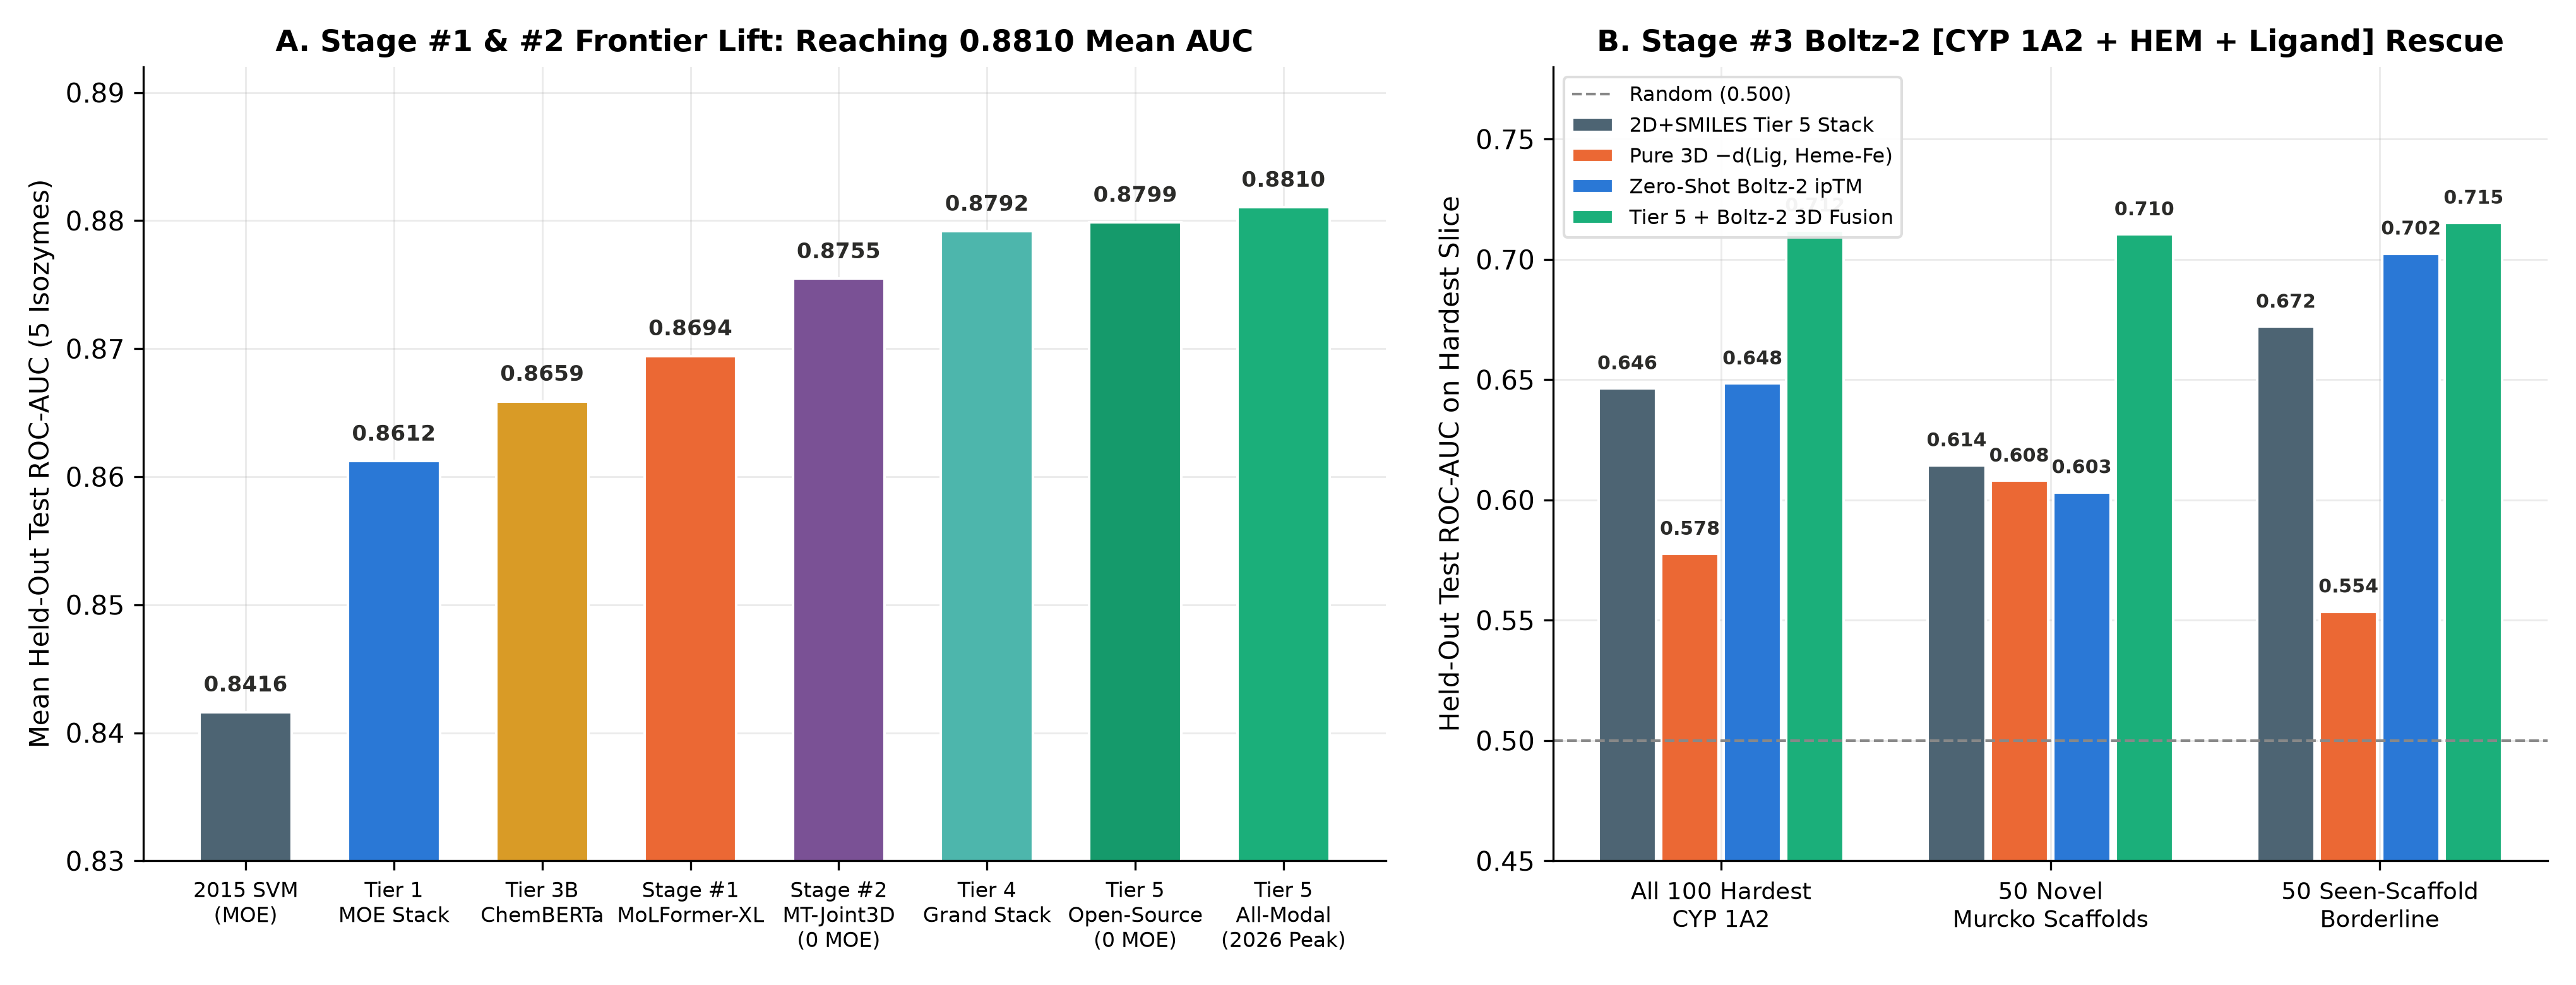
\includegraphics[width=\textwidth]{../extension/img/fig8_tier5_and_boltz2.png}
  \caption{(A) Tier 5 progression reaching 0.8810 mean Test ROC-AUC (0.8799 open-source). (B) Zero-shot \texttt{Boltz-2} \texttt{[CYP 1A2 + HEM + Ligand]} rescue on the 100 hardest CYP 1A2 compounds (+0.0960 AUC on unseen Murcko scaffolds).}
  \label{fig:t5}
\end{figure}

\begin{figure}[htbp]
  \centering
  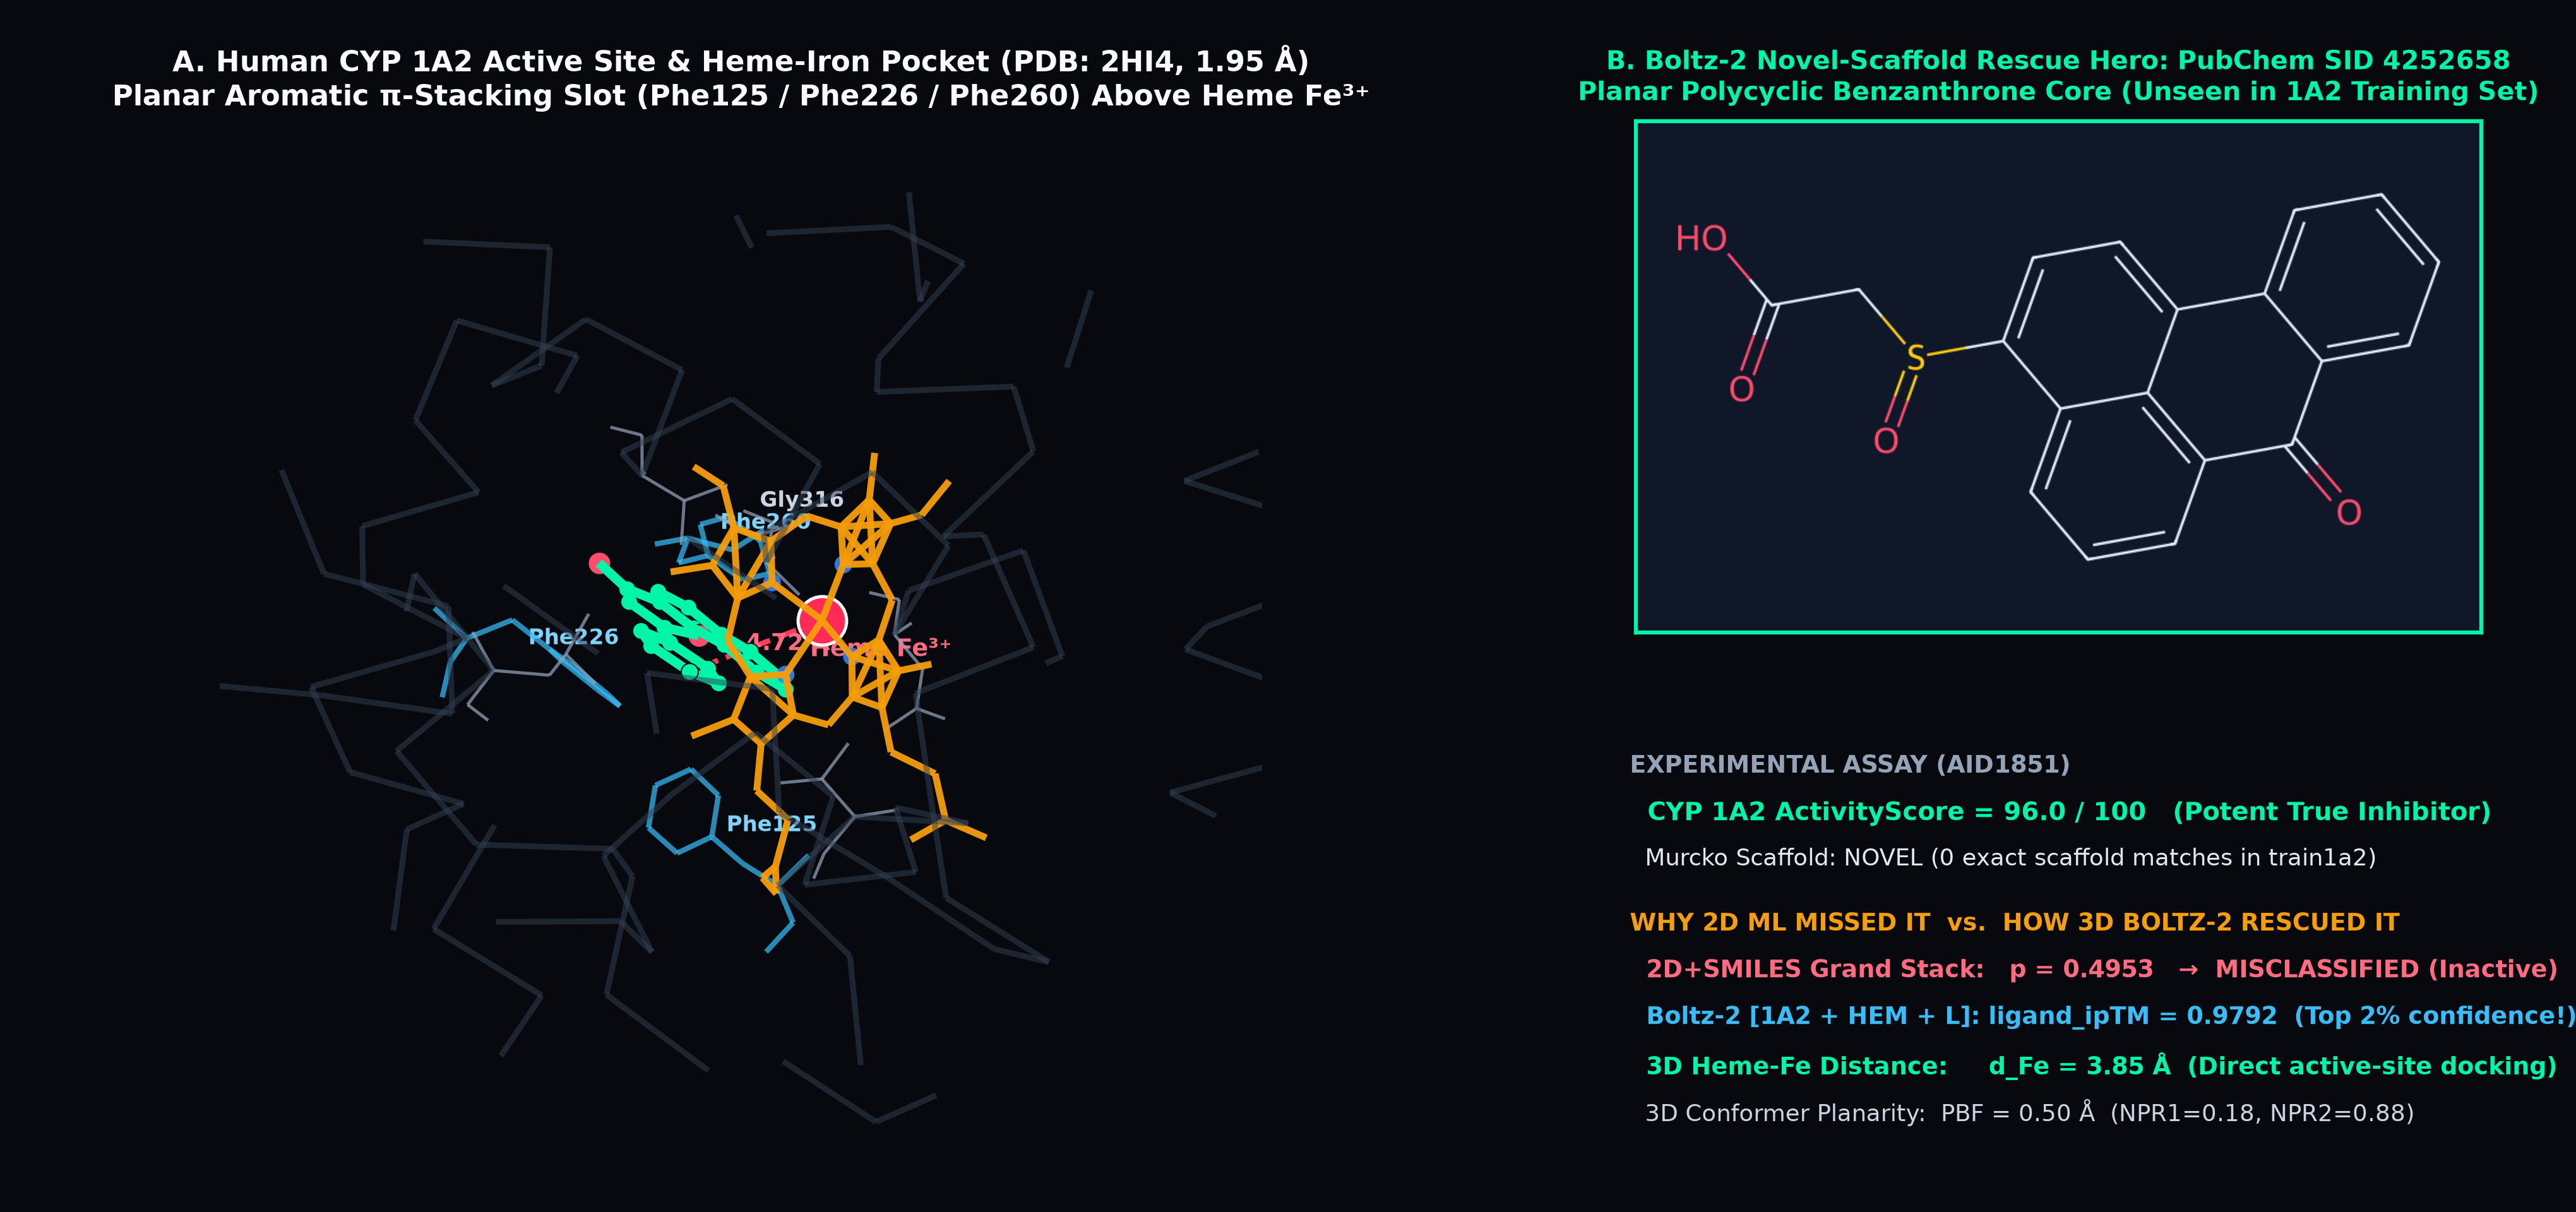
\includegraphics[width=\textwidth]{../extension/img/fig9_cyp1a2_heme_complex.png}
  \caption{(A) Exact atomic coordinates of the human CYP 1A2 active site (\texttt{PDB: 2HI4}, 1.95\,\AA) with Heme $\text{Fe}^{3+}$ and Phe125/Phe226/Phe260 $\pi$-stacking gatekeepers. (B) Novel-scaffold rescue hero \texttt{SID 4252658} (\texttt{ActivityScore = 96.0}).}
  \label{fig:complex}
\end{figure}

\begin{figure}[htbp]
  \centering
  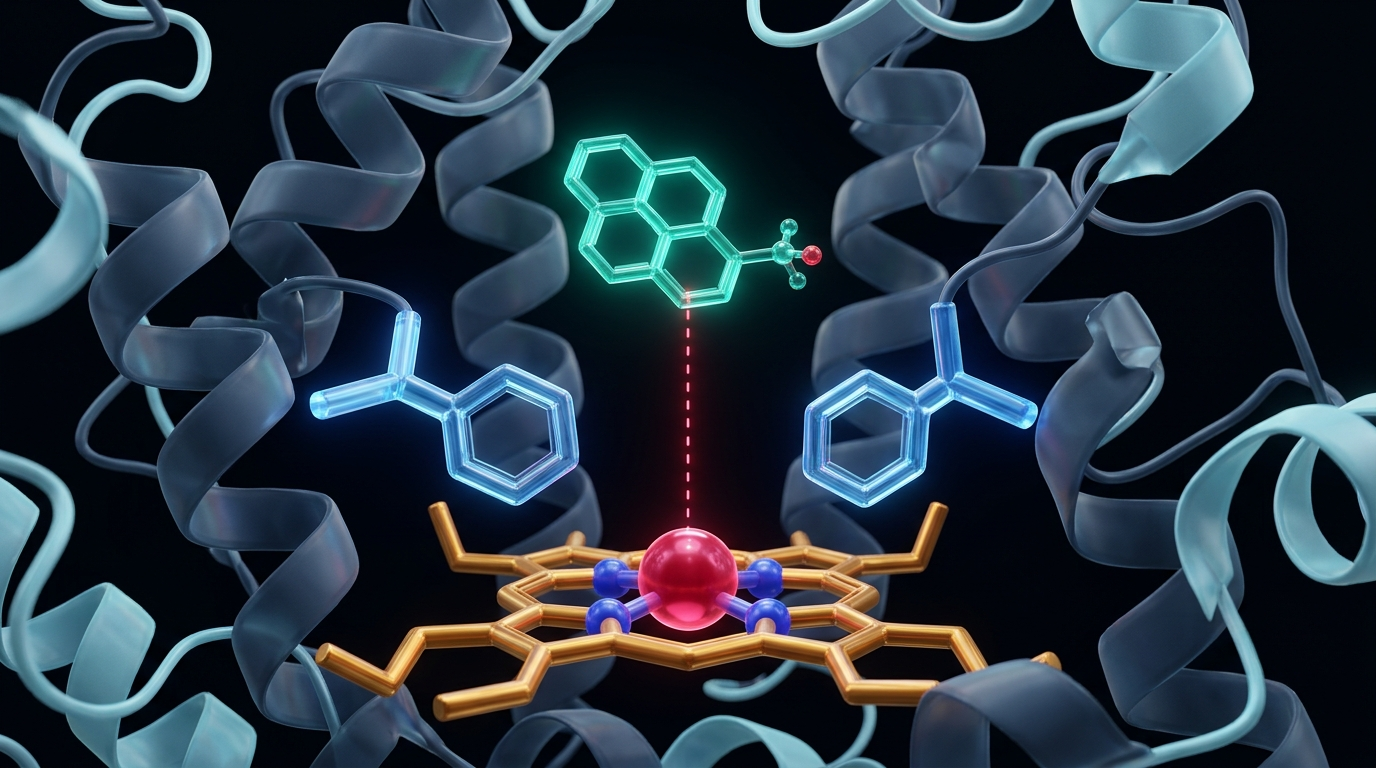
\includegraphics[width=0.92\textwidth]{../extension/img/cyp1a2_pocket_hero.jpg}
  \caption{Conceptual 3D molecular-graphics illustration of the CYP 1A2 active-site pocket: $\alpha$-helical cavity (slate/cyan), flanking phenylalanine aromatic gatekeepers (sky-blue), Heme-b porphyrin with central $\text{Fe}^{3+}$ ion (crimson), and a planar polycyclic inhibitor (emerald) positioned directly above the heme center.}
  \label{fig:hero}
\end{figure}

\section{Practical Blueprint for Modern ADMET Workflows}
These experiments define a clean two-tier architecture for drug-discovery teams: (1)~screen entire compound libraries in milliseconds per molecule using a 100\% open-source stack fusing 2D fingerprints, 3D ETKDGv3 conformers, pretrained chemical language models, and continuous-potency multi-tasking (\textbf{0.8799 AUC}, zero commercial licenses); and (2)~route the top 5--10\% highest-uncertainty or novel-scaffold hits to explicit protein--cofactor--ligand co-folding (\texttt{Boltz-2}), where 3D active-site physics adds nearly +0.10 AUC on unseen scaffolds and yields actionable 3D binding poses for medicinal-chemistry optimization.

\end{document}
